\documentclass[10pt,journal,compsoc]{styles/IEEEtran}
\usepackage{styles/algorithm}
\usepackage[noend]{styles/algorithmic}
\usepackage{graphicx}
\usepackage{color}
\usepackage{listings}
\usepackage{amsmath}
\usepackage[utf8]{inputenc}
\usepackage[T1]{fontenc}
\usepackage[labelformat=empty]{caption}
% *** CITATION PACKAGES ***
\ifCLASSOPTIONcompsoc
  % IEEE Computer Society needs nocompress option
  % requires cite.sty v4.0 or later (November 2003)
  \usepackage[noadjust]{cite}
\else
  % normal IEEE
  \usepackage{cite}
\fi

\title{Tarea 9: M\'etodo BFGS y Gradiente Estoc\'astico}

\author{Juan Gerardo Fuentes Almeida}

% The paper headers
\markboth{Tarea 9: M\'etodo BFGS y Gradiente Estoc\'astico}%
{Shell \MakeLowercase{\textit{et al.}}: Bare Advanced Demo of styles/IEEEtran.cls for Journals}

\IEEEtitleabstractindextext{%
\begin{abstract}
En esta pr\'actica se implementan los algoritmos BFGS y BFGS estoc\'astico para resolver problemas de optimización con Mínimos Cuadrados No Lineales, aplicados a desenvolvimiento de fases.
\end{abstract}
}

\begin{document}

% make the title area
\maketitle

\IEEEdisplaynontitleabstractindextext

\IEEEpeerreviewmaketitle

\section{Introducci\'on}

\IEEEPARstart{E}n Problemas de Mínimos Cuadrados, la función objetivo $f$ tiene la forma especial:\\
 
 $f(x)=\frac{1}{2} \sum \limits_{j=1}^{m} r^2_j (x)$\\
 
donde cada $r_j$ es una función residual suave de $\Re^n$ a $\Re$, esta forma especial hace que el problema sea mas fácil de resolver comparado con un problema general de optimización sin restricciones.\\

Ensamblamos los componentes individuales de $r_j$ en un vector residual $r:\Re^n \rightarrow \Re^m$, de la siguiente manera:\\

$r(x)=(r_1(x),r_2(x),...,r_m(x))^T$\\

Con esta notación, podemos reescribir $f$ como $f(x)=\frac{1}{2} \parallel r^2_j (x) \parallel _2^2$, y sus derivadas en términos del Jacobiano $J(x)$:\\

\begin{figure}[hbtp]
\centering
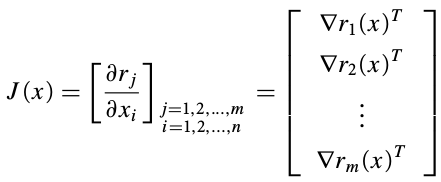
\includegraphics[width=0.35\textwidth]{Jacobian.png}
\caption*{}
\end{figure}

El gradiente y el Hessiano de $f$ se pueden expresar de la siguiente manera:\\

\begin{figure}[hbtp]
\centering
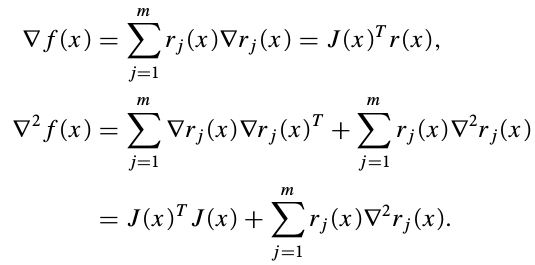
\includegraphics[width=0.4\textwidth]{Hessian.png}
\caption*{}
\end{figure}

En muchas aplicaciones, las primeras derivadas parciales de los residuales, y por tanto, de la Matriz Jacobiana $J(x)$ son relativamente fáciles de calcular. Asimismo, utilizando $J(x)$ podemos calcular el primer t\'ermino $J(x)^T J(x)$ del Hessiano sin evaluar las segundas derivadas de la función $r(x)$, esto es distintivo de los problemas de mínimos cuadrados, ya que los residuos $r_j$ están cerca de la solución, y por tanto, $\nabla^2 r_j (x)$ es relativamente pequeño.\\

\section{Teoría}

\subsection{M\'etodo BFGS}

Es el algoritmo Quasi-Newton m\'as utilizado, se deriva de la optimizaci\'on de la serie de Taylor:

$$m_k(p)=f_k+\nabla f_k^T p+ \frac{1}{2}p^T B_k p$$

Para una matriz $B_k$ sim\'etrica y positiva definida, la cual se actualiza en cada iteraci\'on, como ya antes se ha demostrado, el minimizador para esta función esta dado por:

$$p_k=-B_k^{-1}f_k$$

esta dirección de búsqueda se utiliza para calcular la nueva iteración $x_{k+1}=x_k+\alpha_k p_k$, donde el tamaño de paso $\alpha_k$ satisface las condiciones de Wolfe.\\

Para determinar la siguiente iteración $B_{k+1}$, se impone la siguiente condición, denominada Ecuación Secante:

$$B_{k+1}s_k=y_k$$

Para $s_k=x_{k+1}-x_k$ y $y_k=\nabla f_{k+1}-\nabla f_k$, además, se impone la condición de que esa nueva iteración debe ser lo mas cercana posible a la iteración anterior, lo que equivale a resolver el problema:

$$min_B ||B-B_k||$$

sujeto a $B=B^T$ y $B_{k+1}s_k=y_k$\\

Davidon, Fletcher y Powell en 1959 propusieron la siguiente formula para actualizar la matriz $B_k$:

$$B_{k+1}=(I-\rho_k y_k s_k^T)B_k(I-\rho_k s_k y_k^T)+\rho_k y_k y_k^T$$

con $\rho= 1/y_k^T s_k$, pero después fue sobrepasada por la formula BFGS, en la cual se actualiza la inversa de la matriz $B_k$ denotada como $H_k$:

$$H_{k+1}=(I-\rho_k s_k y_k^T)H_k(I-\rho_k y_k s_k^T)+\rho_k s_k s_k^T$$

\begin{figure}[H]
\centering
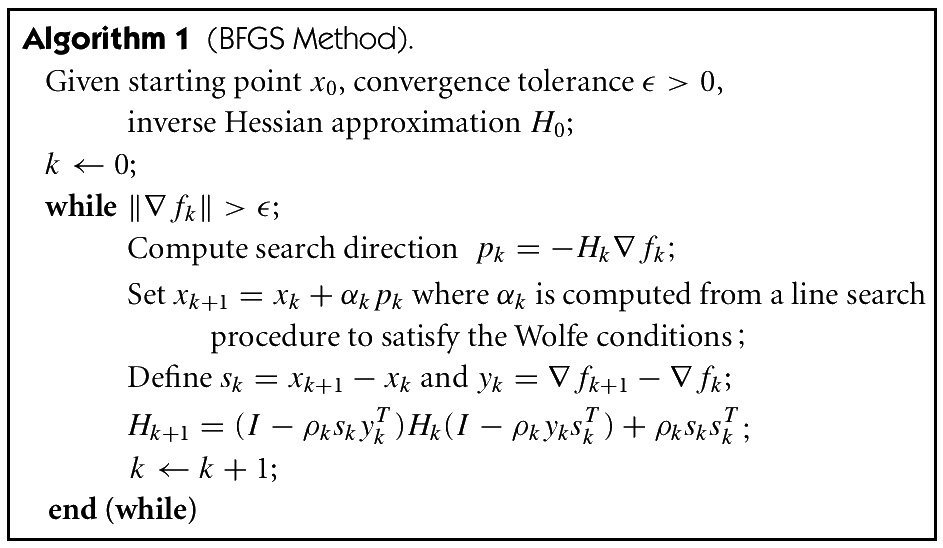
\includegraphics[width=0.5\textwidth]{BFGS.png}
\caption*{}
\end{figure}

\subsection{Gradiente Estocastico}

Si queremos resolver el problema general de optimización:

$$min_{x \in \Re^n} f(x)=\sum_{i=1}^n f_i(x)$$

Sabemos que equivale a resolver:

$$\nabla f(x)=\sum_{i=1}^n \nabla f_i (x)$$

por analogía

$$\nabla f(x)=nE[\nabla f_i (x)]$$

luego podemos interpretar el gradiente de $f(x)$ como una valor esperado y podemos estimarlo sobre una muestra de una población $\textit{U}$:

$$\textit{S}=\textit{U}([1,n],m)$$

con $m<<n$, por tanto podemos definir el Jacobiano del problema de la siguiente manera:

$$\nabla f \simeq \sum_{i \in \textit{S}} \nabla f_i (x) =  \tilde{J}^T \tilde{r}$$


\section{Implementaci\'on}

Sea $f(x)$ la fase desenvuelta de una imagen, y $g(x)$ su fase envuelta, por la propiedad de Nyquist, si la derivada de una función esta acotada en $(-\pi,\pi)$, es decir, $f(x)-f(x-e_1) \in (-\pi,\pi)$, entonces:\\

$f(x)-f(y)=W[g(x)-q(y)]$\\

siendo $W$ el operador de envolvimiento y $\parallel y-x \parallel=1$\\

luego, para recuperar $f(x)$ de $g(x)$, calculamos:\\

$g'_1(x)=g(x)-g(x-e_1)$, $g'_2(x)=g(x)-g(x-e_2)$\\

y envolvemos la función resultante:\\

$\widehat{g'_1(x)}=W[g'_1(x)]$, $\widehat{g'_2(x)}=W[g'_2(x)]$\\

Por tanto, por el criterio de Nyquist, podemos aproximar el residuo entre esta función y la derivada de la fase desenvuelta mediante mínimos cuadrados:\\

$U(f)=\sum \limits_{\Omega} [\widehat{g'_1(x)}-f'_1(x)]^2+\sum \limits_{\Omega} [\widehat{g'_2(x)}-f'_2(x)]^2$\\

donde $f'_1(x)=f(x)-f(x-e_1)$ y $f'_2(x)=f(x)-f(x-e_2)$ son las derivadas de la fase desenvuelta, las cuales podemos aproximar mediante Bases de Funciones Radiales:\\

$f(x)=\sum \limits_{ij} \alpha_{ij} \phi(i,j,x)$

con $\phi(i,j,x)=\exp[\frac{-1}{2\sigma_{ij}}(x-\mu_{ij})^2]$\\

luego\\
$f'_1(x)=\sum \limits_{ij}\alpha_{ij}[\phi(i,j,x)-\phi(i,j,x-e_1)]=\sum \limits_{ij}\alpha_{ij}\varphi_1 (i,j,x)$\\
y $f'_2(x)=\sum \limits_{ij}\alpha_{ij}[\phi(i,j,x)-\phi(i,j,x-e_2)]=\sum \limits_{ij}\alpha_{ij}\varphi_2 (i,j,x)$\\

luego, para recuperar $f(x)$ de $g(x)$, tendremos que minimizar la siguiente expresión:\\

$U(f)=\sum \limits_{\Omega} [\widehat{g'_1(x)}-f'_1(x)]^2+\sum \limits_{\Omega} [\widehat{g'_2(x)}-f'_2(x)]^2$\\

\subsection{Optimización de $\alpha$}

Para optimizar el valor de $\alpha$, el cual es la amplitud de las funciones radiales, se construye un Jacobiano cuyas filas son los componentes en $x$ y en $y$ de la función objetivo (2 veces el numero de pixeles de la imagen)\\

\[J(\alpha)= \left( \begin{array}{cccc}
\frac{\partial r(x_1)}{\partial \alpha_1} & \frac{\partial r(x_1)}{\partial \alpha_2} & \ldots & \frac{\partial r(x_1)}{\partial \alpha_m} \\
\vdots & \vdots & \ddots & \vdots \\
\frac{\partial r(x_N)}{\partial \alpha_1} & \frac{\partial r(y_N)}{\partial \alpha_2} & \ldots & \frac{\partial r(x_N)}{\partial \alpha_m} \\
\frac{\partial r(y_1)}{\partial \alpha_1} & \frac{\partial r(y_1)}{\partial \alpha_2} & \ldots & \frac{\partial r(y_1)}{\partial \alpha_m} \\
\vdots & \vdots & \ddots & \vdots \\
\frac{\partial r(y_N)}{\partial \alpha_1} & \frac{\partial r(y_N)}{\partial \alpha_2} & \ldots & \frac{\partial r(y_N)}{\partial \alpha_m} 
\end{array} \right)\] 

El gradiente de la función esta determinado por $J_k^Tr_k$.\\

Cada elemento de esta matriz esta definido por la siguiente expresión:\\

$\frac{\partial r(x_k)}{\partial \alpha_{ij}}=-\varphi_1(i,j,x_k)=-\frac{(x_{k_1}-\mu_{ij_1})}{\sigma_{ij}^2}\phi(i,j,x_k)$\\

$\frac{\partial r(y_k)}{\partial \alpha_{ij}}=-\varphi_2(i,j,x_k)=-\frac{(x_{k_2}-\mu_{ij_2})}{\sigma_{ij}^2}\phi(i,j,x_k)$\\

\subsection{Optimización de $\mu$}

Para optimizar el valor de $\mu$, el cual es la media de las funciones radiales, se construye un Jacobiano cuyas filas son los componentes en $x$ y en $y$ de la función objetivo (2 veces el numero de pixeles de la imagen), y cuyas columnas están repartidas entre las componentes en x y en y de la medias (2 veces el numero de funciones radiales):\\

\[J(\mu)= \left( \begin{array}{cccccc}
\frac{\partial r(x_1)}{\partial \mu(x_1)} & \ldots & \frac{\partial r(x_1)}{\partial \mu(x_m)} & \frac{\partial r(x_1)}{\partial \mu(y_1)} & \ldots & \frac{\partial r(x_1)}{\partial \mu(x_m)} \\
\vdots & \ddots & \vdots & \vdots & \ddots & \vdots \\

\frac{\partial r(x_N)}{\partial \mu(x_1)} & \ldots & \frac{\partial r(x_N)}{\partial \mu(x_m)} & \frac{\partial r(x_N)}{\partial \mu(y_1)} & \ldots & \frac{\partial r(x_N)}{\partial \mu(x_m)} \\
\frac{\partial r(y_1)}{\partial \mu(x_1)} & \ldots & \frac{\partial r(y_1)}{\partial \mu(x_m)} & \frac{\partial r(y_1)}{\partial \mu(y_1)} & \ldots & \frac{\partial r(y_1)}{\partial \mu(x_m)} \\
\vdots & \ddots & \vdots & \vdots & \ddots & \vdots \\

\frac{\partial r(y_N)}{\partial \mu(x_1)} & \ldots & \frac{\partial r(y_N)}{\partial \mu(x_m)} & \frac{\partial r(y_N)}{\partial \mu(y_1)} & \ldots & \frac{\partial r(y_N)}{\partial \mu(x_m)}
\end{array} \right)\] 

El gradiente de la función esta determinado por $J_k^Tr_k$. 

Cada elemento de esta matriz esta definido por la siguiente expresión:\\

\small 
$\frac{\partial r(x_k)}{\partial \mu(x_{ij})}=- \alpha_{ij} \frac{\partial \varphi_1(i,j,x_k)}{\partial \mu(x_{ij})} =- \frac{\alpha_{ij}}{\sigma_{ij}^2}\phi(i,j,x_k)[1-\frac{(x_{k_1}-\mu_{ij_1})^2}{\sigma_{ij}^2}] $\\
\normalsize

$\frac{\partial r(x_k)}{\partial \mu(y_{ij})}= \frac{\alpha_{ij}}{\sigma_{ij}^4}\phi(i,j,x_k)(x_{k_1}-\mu_{ij_1})(x_{k_2}-\mu_{ij_2})$\\

$\frac{\partial r(y_k)}{\partial \mu(x_{ij})}=\frac{\alpha_{ij}}{\sigma_{ij}^4}\phi(i,j,x_k)(x_{k_1}-\mu_{ij_1})(x_{k_2}-\mu_{ij_2})$\\

\small 
$\frac{\partial r(y_k)}{\partial \mu(y_{ij})}=- \alpha_{ij} \frac{\partial \varphi_1(i,j,x_k)}{\partial \mu(y_{ij})} =- \frac{\alpha_{ij}}{\sigma_{ij}^2}\phi(i,j,x_k)[1-\frac{(x_{k_2}-\mu_{ij_2})^2}{\sigma_{ij}^2}] $\\
\normalsize

\subsection{Optimización de $\sigma$}

Para optimizar el valor de $\sigma$, el cual es la desviación estándar de las funciones radiales, se construye un Jacobiano cuyas filas son los componentes en $x$ y en $y$ de la función objetivo (2 veces el numero de pixeles de la imagen)\\

\[J(\alpha)= \left( \begin{array}{cccc}
\frac{\partial r(x_1)}{\partial \sigma_1} & \frac{\partial r(x_1)}{\partial \sigma_2} & \ldots & \frac{\partial r(x_1)}{\partial \sigma_m} \\
\vdots & \vdots & \ddots & \vdots \\
\frac{\partial r(x_N)}{\partial \sigma_1} & \frac{\partial r(y_N)}{\partial \sigma_2} & \ldots & \frac{\partial r(x_N)}{\partial \sigma_m} \\
\frac{\partial r(y_1)}{\partial \sigma_1} & \frac{\partial r(y_1)}{\partial \sigma_2} & \ldots & \frac{\partial r(y_1)}{\partial \sigma_m} \\
\vdots & \vdots & \ddots & \vdots \\
\frac{\partial r(y_N)}{\partial \sigma_1} & \frac{\partial r(y_N)}{\partial \sigma_2} & \ldots & \frac{\partial r(y_N)}{\partial \sigma_m} 
\end{array} \right)\] 

El gradiente de la función esta determinado por $J_k^Tr_k$. 

Cada elemento de esta matriz esta definido por la siguiente expresión:\\

$\frac{\partial r(x_k)}{\partial \sigma_{ij}}=-\frac{\alpha_{ij}}{\sigma_{ij}^3}(x_{k_1}-\mu_{ij_1})\phi(i,j,x_k)[2-\frac{(x_k-\mu_{ij})^2}{\sigma_{ij}}]$\\

$\frac{\partial r(y_k)}{\partial \sigma_{ij}}=-\frac{\alpha_{ij}}{\sigma_{ij}^3}(x_{k_2}-\mu_{ij_2})\phi(i,j,x_k)[2-\frac{(x_k-\mu_{ij})^2}{\sigma_{ij}}]$\\

\section{Resultados}

A continuación se muestran las imágenes que se obtuvieron durante la ejecución de la práctica, para diferente n\'umero de funciones radiales en una imagen de prueba, utilizando los métodos de BFGS y BFGS con gradiente estocástico:\\


\begin{figure}[H]
\centering

\includegraphics[width=0.25\textwidth]{phase.png}
\caption{Imagen Desenvuelta}
\end{figure}

Los siguientes resultados fueron obtenidos con el método BFGS:\\

\begin{figure}[H]
	\centering
	
\includegraphics[width=0.15\textwidth]{BFGS1.png}
	
\includegraphics[width=0.15\textwidth]{BFGS2.png}
	
\includegraphics[width=0.15\textwidth]{BFGS3.png}
	
	\caption{De derecha a izquierda: Resultados para 1, 4 y 9 funciones radiales.}
\end{figure}

\begin{figure}[H]
	\centering
	
\includegraphics[width=0.15\textwidth]{BFGS4.png}
	
\includegraphics[width=0.15\textwidth]{BFGS5.png}
	
\includegraphics[width=0.15\textwidth]{BFGS6.png}
	
	\caption{De derecha a izquierda: Resultados para 16, 25 y 36 funciones radiales. }
\end{figure}

Los siguientes resultados fueron obtenidos con el método SGD:\\

\begin{figure}[H]
	\centering
	
\includegraphics[width=0.15\textwidth]{SGD1.png}
	
\includegraphics[width=0.15\textwidth]{SGD2.png}
	
\includegraphics[width=0.15\textwidth]{SGD3.png}
	
	\caption{De derecha a izquierda: Resultados para 1, 4 y 9 funciones radiales.}
\end{figure}

\section{Conclusiones}

La siguiente tabla muestra el desempeño de los algoritmos implementados en esta pr\'actica, para diferente numero de RBF's. Como se observa, el algoritmo SGD, que fue implementado para una muestra del 50 por ciento, en general realiza m\'as iteraciones, lo que afecta directamente en el tiempo de ejecución, esto result\'o contraproducente, ya que como se definió el criterio de paro en función de la razón de cambio entre la evaluación de la función objetivo, el algoritmo sigue iterando cuando el resultado todavía puede ser mejorado, por lo que no se observo ninguna mejora al implementarse el método estocástico.

\begin{figure}[H]
\centering
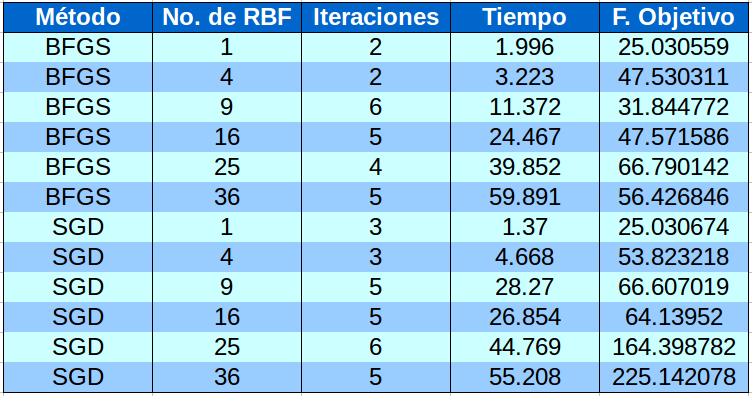
\includegraphics[width=0.5\textwidth]{tabla.png}
\caption{Desempeño de los métodos BFGS y SGD}
\end{figure}
\bibliographystyle{plain}
\bibliography{biblio}


\appendix
\section{Implementation details}
El programa est\'a implementado tomando en cuenta todas estandarizaciones indicadas en el curso.

El \textit{makefile} que se ha generado, incluye los comandos \textit{make}, \textit{run}, \textit{test} y \textit{clean}. El programa recibe el nombre del archivo de la imagen y el parámetro \textit{methodID}, el cual indica al programa que método de optimización se va a usar, 1 para BFGS y 2 para SGD, el comando \textit{test} ejecuta 20 iteraciones del método de BFGS con 4 gaussianas.\\

\begin{figure}[H]
\centering
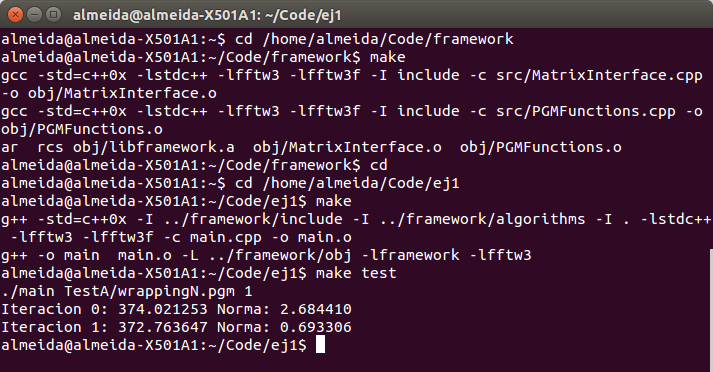
\includegraphics[width=0.5\textwidth]{screen.png}
\caption*{}
\end{figure}

\end{document}


